\whiteBGstarBegin
\setcounter{section}{0}
\section{Lý thuyết: Thấu kính mỏng và tính chất quang học của thấu kính mỏng}
\begin{enumerate}[label=\bfseries Câu \arabic*:]
	
	\item \mkstar{1} [15]
	
	\cauhoi{
		
	Thấu kính mỏng là gì? Phân loại và nêu một số ứng dụng của thấu kính mỏng trong cuộc sống. 
		
	}
	
	\loigiai{
		
		- Thấu kính là một khối chất trong suốt giới hạn bởi hai mặt cong hoặc một mặt cong và một mặt phẳng.
		
		- Có hai loại: thấu kính hội tụ (rìa mỏng) và thấu kính phân kì (rìa dày).
		
		- Ứng dụng: kính khắc phục tật của mắt (kính cận, lão...), máy chiếu,...
	}
	
	\item \mkstar{1} [18]
	
	\cauhoi{
		Nêu tính chất quang học của quang tâm, tiêu điểm ảnh chính, tiêu điểm vật chính của thấu kính phân kỳ. Minh họa bằng đường truyền tia sáng cho mỗi trường hợp.
		
		
	}
	
	\loigiai{
		
		 Mọi tia sáng tới qua quang tâm O đều truyền thẳng qua thấu kính. Hình vẽ:
		 
		 \begin{center}
		 	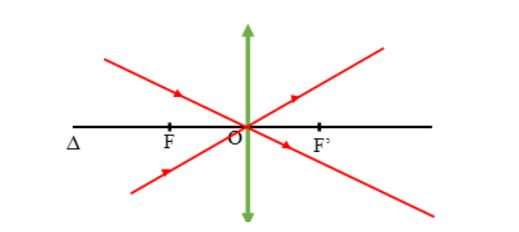
\includegraphics[scale=0.9]{../figs//VN11-2021-PH-TP028-10.JPG}
		 \end{center}
	 
	 	Mọi tia sáng tới song song với trục chính là tia ló sẽ qua tiêu điểm ảnh F’ ( đối với thấu kính hội tụ) hay có đường kéo dài qua tiêu điểm ảnh F’ ( đối với thấu kính phân kì). Hình vẽ:
	 	
	 	\begin{center}
	 		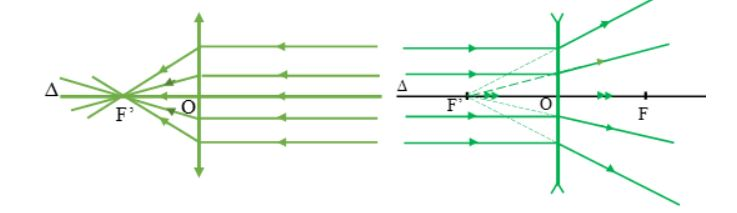
\includegraphics[scale=0.9]{../figs//VN11-2021-PH-TP028-11.JPG}
	 	\end{center}
 	
 		Mọi tia sáng tới qua tiêu điểm vật F (đối với thấu kính hội tụ) hay có đường kéo dài qua tiêu điểm vật F (đối với thấu kính phân kì) thì tia ló sẽ song song với trục chính. Hình vẽ:
 		
 		\begin{center}
 			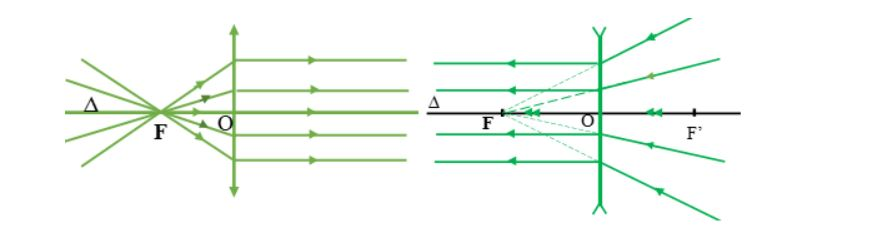
\includegraphics[scale=0.9]{../figs//VN11-2021-PH-TP028-12.JPG}
 		\end{center}
	}
	
	\item \mkstar{1} [20]
	
	\cauhoi{
		
		Vật thật đặt trước thấu kính phân kỳ sẽ cho ảnh có tính chất như thế nào?
		
	}
	
	\loigiai{		
		
	Thấu kính phân kì: vật thật luôn cho ảnh ảo, nhỏ hơn vật, cùng chiều vật.
		
	}
	
	

\end{enumerate}
\section{Lý thuyết: Đường đi của tia sáng qua thấu kính và vẽ ảnh tạo bởi thấu kính}
\begin{enumerate}[label=\bfseries Câu \arabic*:]
	
		\item \mkstar{1} [32]
	
	\cauhoi{
		
		Tìm hình vẽ đúng về đường truyền tia sáng qua quang tâm O của thấu kính
		
		\begin{mcq}(2)
			\item \begin{center}
				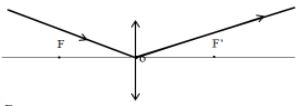
\includegraphics[scale=0.9]{../figs//VN11-2021-PH-TP028-14.JPG}
			\end{center}
			\item \begin{center}
				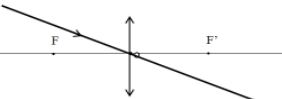
\includegraphics[scale=0.9]{../figs//VN11-2021-PH-TP028-15.JPG}
			\end{center}
			\item \begin{center}
				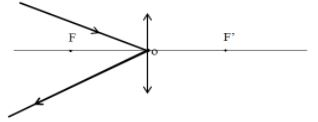
\includegraphics[scale=0.9]{../figs//VN11-2021-PH-TP028-16.JPG}
			\end{center}
			\item \begin{center}
				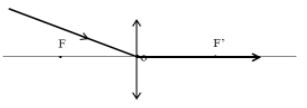
\includegraphics[scale=0.9]{../figs//VN11-2021-PH-TP028-17.JPG}
			\end{center}
			
		\end{mcq}
	}
	
	\loigiai{
		\textbf{Đáp án: B.}
	}
	\item \mkstar{1} [32]

	\cauhoi{

		Tìm hình vẽ đúng về đường truyền tia sáng qua các thấu kính sau:
		
		
		\begin{mcq}(2)
			\item \begin{center}
				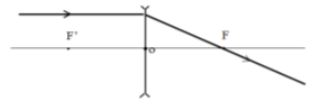
\includegraphics[scale=0.9]{../figs//VN11-2021-PH-TP028-18.JPG}
			\end{center}
			\item \begin{center}
				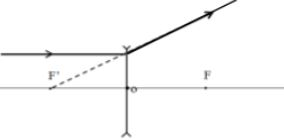
\includegraphics[scale=0.9]{../figs//VN11-2021-PH-TP028-19.JPG}
			\end{center}
			\item \begin{center}
				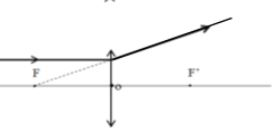
\includegraphics[scale=0.9]{../figs//VN11-2021-PH-TP028-20.JPG}
			\end{center}
			\item \begin{center}
				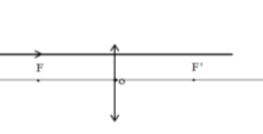
\includegraphics[scale=0.9]{../figs//VN11-2021-PH-TP028-21.JPG}
			\end{center}
			
		\end{mcq}
	}
		\loigiai{
			
			\textbf{Đáp án: B.}
		
	}
		\item \mkstar{2} [21]
	
	\cauhoi{
		Vật sáng AB đặt vuông góc với trục chính của thấu kính, cách thấu kính một khoảng $\SI{40}{cm}$ cho một ảnh trước thấu kính $\SI{20}{cm}$. Đây là
		
		\begin{mcq}(2)
			\item thấu kính hội tụ có tiêu cự $\SI{40}{cm}$.	
			\item thấu kính phân kì có tiêu cự $\SI{40}{cm}$.
			\item thấu kính hội tụ có tiêu cự $\SI{20}{cm}$.	
			\item thấu kính phân kì có tiêu cự $\SI{20}{cm}$.
		\end{mcq}
	}
	
	\loigiai{
		\textbf{Đáp án: B.}
		
		Ta có: $d = \SI{40}{cm}$.
		
		Do ảnh trước thấu kính nên $d'=-\SI{20}{cm}$ 
		
		$$\dfrac{1}{f} = \dfrac{1}{d} + \dfrac{1}{d'} = - \dfrac{1}{40} \Rightarrow f = -\SI{40}{cm}.$$
		
		Thấu kính đã cho là thấu kính phân kì do ảnh trước thấu kính và có $f = -\SI{40}{cm}$. 
	}
	
	\item \mkstar{1} [10]

\cauhoi{
	
	Thấu kính là gì? Khi vật sáng AB đặt vuông góc trên trục chính của một thấu kính  luôn cho ảnh ảo thì đó là thấu kính gì? Ảnh này có chiều và độ lớn như thế nào so với vật?
	
	
}

\loigiai{
	
	Thấu kính là một khối chất trong suốt được giới hạn bởi hai mặt cong hoặc một mặt cong một mặt phẳng.
	
	Thấu kính phân kỳ luôn cho ảnh ảo, cùng chiều và nhỏ hơn vật.
	
	
}

\item \mkstar{1} [36]

\cauhoi{
	Điền vào chỗ trống sau đây: 
	
	* Quang tâm:
	
	+ Điểm O chính giữa của thấu kính mà mọi tia sáng truyền qua O đều $\ldots$ (1) $\ldots$ gọi là quang tâm của thấu kính.
	
	+ Đường thẳng đi qua quang tâm O và $\ldots$ (2) $\ldots$ với mặt thấu kính là trục chính.
	
	+ Các đường thẳng khác qua quang tâm O  là $\ldots$ (3) $\ldots$.
	
	* Mỗi thấu kính có 2 tiêu điểm: tiêu điểm $\ldots$ (4) $\ldots$ và tiêu điểm ảnh (F’) $\ldots$ (5) $\ldots$ nhau qua quang tâm O.
	
	+ Tiêu điểm ảnh F’: Chiếu đến thấu kính 1 chùm tia tới $\ldots$ (6) $\ldots$ thì ta nhận được chùm tia ló cắt nhau tại 1 điểm trên trục tương ứng với chùm tia tới. Điểm này gọi là $\ldots$ (7) $\ldots$.
	
	+ Tiêu điểm vật F: Chùm tia tới xuất phát từ điểm F cho tia ló $\ldots$ (8) $\ldots$.
	
}

\loigiai{
	
	(1): truyền thẳng.
	
	(2): vuông góc.
	
	(3): trục phụ.
	
	(4): vật (F).
	
	(5): đối xứng
	
	(6): song song.
	
	(7): tiêu điểm ảnh.
	
	(8): song song.
}	

		\item \mkstar{2} [15]
	
	\cauhoi{
		
		Một thấu kính phân kỳ có tiêu cự $-\SI{40}{cm}$. Vật sáng AB đặt vuông góc trục chính và cách thấu kính một đoạn $\SI{20}{cm}$. Vẽ ảnh và nêu tính chất ảnh.
		
	}
	\loigiai{
		
		Vị trí ảnh
		
		$$\dfrac{1}{f} = \dfrac{1}{d} + \dfrac{1}{d'} \Rightarrow d' = - \dfrac{40}{3}.$$
		
		Độ phóng đại
		
		$$ k= - \dfrac{d'}{d}= \dfrac{2}{3}.$$
		
		Vì đây là thấu kính phân kì nên ảnh là ảnh ảo, nhỏ hơn vật và cùng chiều vật.
		
		\begin{center}
			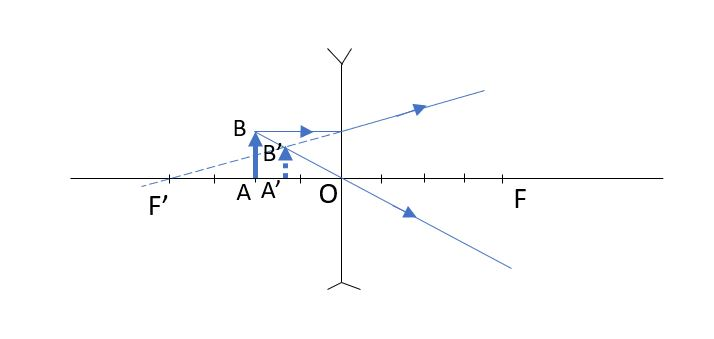
\includegraphics[scale=0.9]{../figs//VN11-2021-PH-TP032-06.JPG}
		\end{center}
	}
	\item \mkstar{2} [16]
	
	\cauhoi{
		
		Một thấu kính hội tụ có tiêu cự $\SI{40}{cm}$. Vật sáng AB cao $\SI{10}{cm}$ đặt vuông góc với trục chính của thấu kính và cách thấu kính $\SI{60}{cm}$. Hãy dựng ảnh của vật sáng AB qua thấu kính.
		
		
	}
	\loigiai{
		
	Vị trí của ảnh
		
		$$\dfrac{f} =\dfrac{1}{d} + \dfrac{1}{d'}  \Rightarrow d ' = \SI{120}{cm}.$$
		
		Độ phóng đại của thấu kính
		
		$$ k = - \dfrac{d}{d'} = -2.$$
		
		\begin{center}
			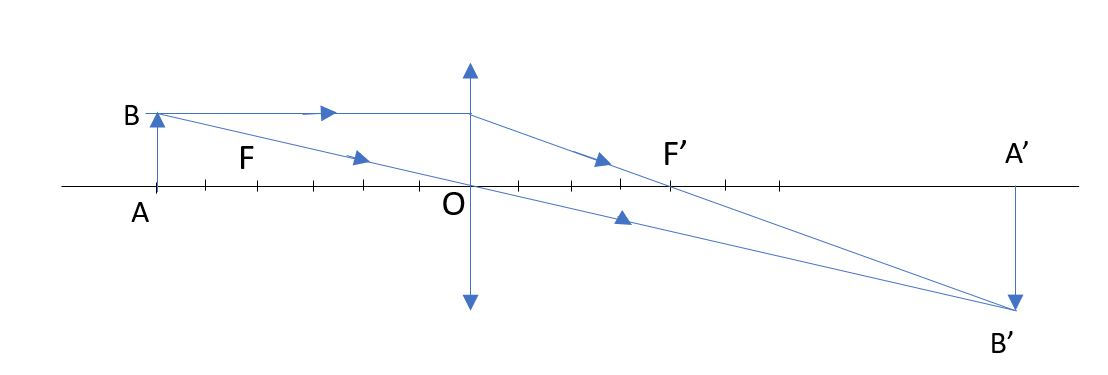
\includegraphics[scale=0.6]{../figs//VN11-2021-PH-TP032-07.JPG}
		\end{center}
	}
	\item \mkstar{2} [23]
	
	\cauhoi{
		
		Một thấu kính hội tụ có độ tụ $D = \SI{5}{dp}$. Đặt một vật sáng AB có chiều cao $\SI{2}{cm}$ trước thấu kính $\SI{40}{cm}$. Vẽ hình.
		
	}
	\loigiai{
		
		Tiêu cự của thấu kính
		
		$$f = \dfrac{1}{D} = \SI{20}{cm}.$$
		
		Vị trí của ảnh
		
		$$\dfrac{1}{d'} = \dfrac{1}{f} - \dfrac{1}{d} \Rightarrow d' = \SI{40}{cm}.$$
		
		Độ phóng đại của thấu kính
		
		$$ k =  - \dfrac{d'}{d} = -1.$$
		
		\begin{center}
			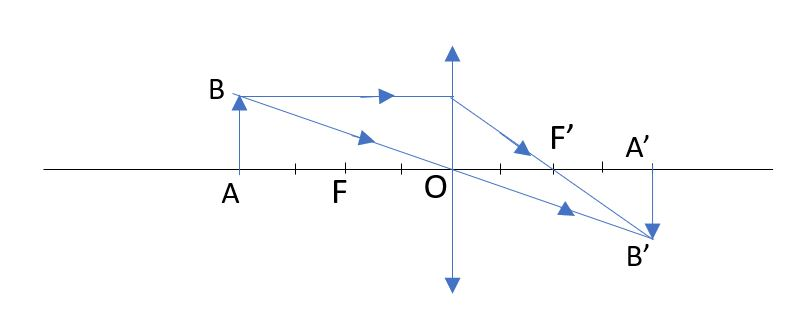
\includegraphics[scale=0.6]{../figs//VN11-2021-PH-TP032-08.JPG}
		\end{center}
	}

	\item \mkstar{2} [33]
	
	\cauhoi{
		
		Vật thật AB được đặt trên trục chính của thấu kính hội tụ có tiêu cự $\SI{20}{cm}$. Khoảng cách từ vật đến thấu kính là $\SI{30}{cm}$. Hãy xác định tính chất, chiều, độ lớn của ảnh, vẽ ảnh.
		
		
	}
	\loigiai{
		
		Vị trí ảnh
		
		$$\dfrac{1}{d'} = \dfrac{1}{f} - \dfrac{1}{d} \Rightarrow d' = \SI{60}{cm}.$$
		
		Độ phóng đại của thấu kính
		
		$$ k = - \dfrac{d'}{d} = -2 <0.$$
		
		Suy ra đây là ảnh thật, ngược chiều vật và cao gấp 2 lần vật.
		
		\begin{center}
			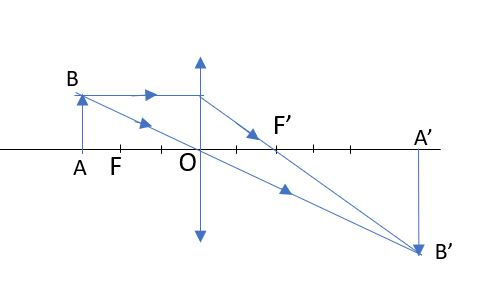
\includegraphics[scale=0.9]{../figs//VN11-2021-PH-TP032-09.JPG}
		\end{center}
	}

		\item \mkstar{2} [28]
	
	\cauhoi{
		
		
		\begin{enumerate}[label=\alph*)]
			\item Hình vẽ bên (Hình 1) biểu diễn loại thấu kính gì? Cho biết vì sao nó có tên gọi như vậy?
			\begin{center}
				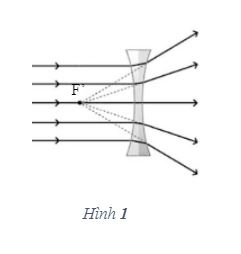
\includegraphics[scale=0.9]{../figs//VN11-2021-PH-TP028-13.JPG}
			\end{center}
			
			\item Cho khoảng cách từ quang tâm O đến một tiêu điểm chính của một thấu kính phân kỳ là $\SI{20}{cm}$. Đặt một vật sáng AB vuông góc với trục chính của thấu kính và cách thấu kính một đoạn $\SI{60}{cm}$. Xác định tiêu cự của thấu kính. Xác định vị trí, tính chất của ảnh và độ phóng đại. Vẽ hình (đúng tỉ lệ).
			\end{enumerate}
		
	}
	\loigiai{
		
		
		\begin{enumerate}[label=\alph*)]
			\item Thấu kính phân kì/thấu kính rìa dày/thấu kính lõm.
			
			Vì: nó làm phân kì chùm sáng tới song song/nó có phần rìa dày hơn phần giữa/nó có phần giữa lõm.
			
			\item Tiêu cự của thấu kính: $f = - \SI{20}{cm}.$
			
			Vị trí của ảnh: 
			
			$$d'=\dfrac{df}{d-f} =-\SI{15}{cm}.$$
			
			Tính chất của ảnh: ảnh ảo (do $d’ < 0$) 
			
			Độ phóng đại:
			
			$$k= - \dfrac{d'}{d} =\text{0,25}.$$ 
			
			
			\begin{center}
				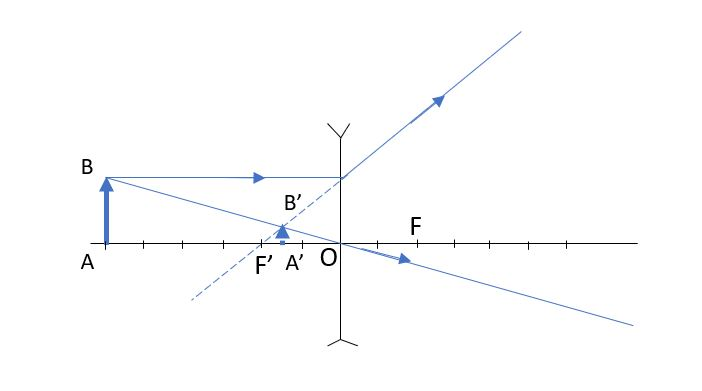
\includegraphics[scale=0.9]{../figs//VN11-2021-PH-TP032-10.JPG}
			\end{center}
		\end{enumerate}
		
			
		
	}

	\item \mkstar{2} [10]
	
	\cauhoi{
		
		Một vật thật AB cao $\SI{10}{cm}$ đặt vuông góc trục chính của thấu kính có tiêu cự $f$ cho ảnh ảo A$_1$B$_1$ cao $\SI{20}{cm}$, ảnh cách thấu kính $\SI{10}{cm}$. Đây là thấu kính gì? Tiêu cự bằng bao nhiêu? Vẽ ảnh của vật qua thấu kính theo đúng tỉ lệ.
		
	}
	\loigiai{
		
			Ta có:
			
			$$ |k| = \dfrac{A_1B_1}{AB} = 2.$$
			
			Đây là thấu kính hội tụ do vật thật cho ảnh ảo lớn hơn vật, nên $ k>0$
			
			$$ k = - \dfrac{d'}{d}  \Rightarrow d = -\dfrac{d'}{k} = \SI{5}{cm} \ (d' = - \SI{10}{cm}).$$

			Tiêu cự của thấu kính 
			
			$$\dfrac{1}{f} = \dfrac{1}{d} + \dfrac{1}{d'} \Rightarrow f = \SI{10}{cm}.$$
			
			
			\begin{center}
				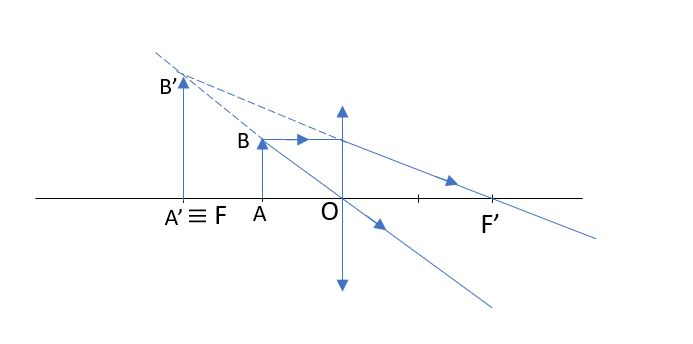
\includegraphics[scale=0.9]{../figs//VN11-2021-PH-TP032-11.JPG}
			\end{center}

}

\end{enumerate}

\section{Lý thuyết: Xác định vị trí, tính chất, độ lớn của vật và ảnh}
\begin{enumerate}[label=\bfseries Câu \arabic*:]
	
	\item \mkstar{1} [21]
	
	\cauhoi{
		Gọi $d$ là khoảng cách từ vật tới thấu kính, $d’$ là khoảng cách từ ảnh đến thấu kính và $f$ là tiêu cự của thấu kính. Độ phóng đại ảnh qua thấu kính là
		
		\begin{mcq}(2)
			\item $k = -\dfrac{d'}{d}.$
			\item $k = \dfrac{f}{f-d}.$
			\item $k = -\dfrac{f-d'}{f}.$
			\item Cả A, B, C đều đúng.
		\end{mcq}
		
		
	}
	\loigiai{
		
		\textbf{Đáp án: D.}
		
		Độ phóng đại ảnh qua thấu kính là $k = -\dfrac{d'}{d}.$
		
		Mà $$ \dfrac{1}{f} =\dfrac{1}{d} + \dfrac{1}{d'}.$$
	}
	\item \mkstar{1} [26]
	
	\cauhoi{
	Viết công thức liên hệ giữa tiêu cự, vị trí vật và vị trí ảnh. Cho biết quy ước về dấu của các đại lượng trong công thức.
	
	}
	\loigiai{
		
	* Công thức liên hệ giữa vị trí các vật và ảnh:  
	
	$$\dfrac{1}{f} = \dfrac{1}{d} +\dfrac{1}{d'}.$$
	
	* Quy ước: 
	
	 $f > 0$: thấu kính hội tụ; $f < 0$: thấu kính phân kì.
	
	 $d > 0$: Vật thật; $d < 0$: Vật ảo.
	
	 $d’ > 0$: ảnh thật; $d’ < 0$: Ảnh ảo.
	
	
	}
	\item \mkstar{2} [6]
	
	\cauhoi{
		
		Vật sáng AB đặt vuông góc với một trục chính của một thấu kính có tiêu cự $\SI{30}{cm}$ cho ảnh A’B’ = 3AB rõ nét trên màn. Xác định vị trí vật và ảnh. Vẽ ảnh minh họa.
		
	}
	\loigiai{
		
		Ta có:
		
		$$ |k| = \dfrac{\text{A'B'}}{\text{AB}} = 3.$$
		
		Mà ảnh hứng được trên màn là ảnh thật nên thấu kính này là thấu kính hội tụ, và ảnh thật ngược chiều vật và lớn hơn vật. $k < 0$
		
		$$ 3 = \left|-\dfrac{d'}{d}\right| \Rightarrow d' = 3d.$$
		
		Lại có:
		
		$$f = \dfrac{dd'}{d+d'} = 30.$$
		
		Suy ra $d = \SI{40}{cm}.$ và $d' = \SI{120}{cm}.$
		
		
		\begin{center}
			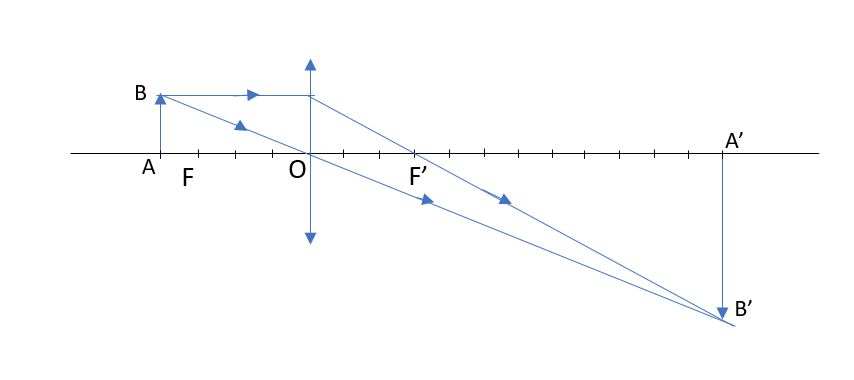
\includegraphics[scale=0.9]{../figs//VN11-2021-PH-TP032-12.JPG}
		\end{center}
		 
	}
	\item \mkstar{2} [7]
	
	\cauhoi{
		
		Một thấu kính hội tụ có tiêu cự $\SI{40}{cm}$. Vật sáng là đoạn thẳng AB đặt vuông góc với trục chính cách thấu kính $\SI{20}{cm}$. Xác định vị trí, tính chất ảnh A’B’ của AB.
		
		
	}
	\loigiai{
		
		+ Ta có: 
		
		$$d' = \dfrac{df}{d-f} = -\SI{40}{cm}.$$
		
		Do $d' <0$ nên đây là ảnh ảo.
		
		+ Độ phóng đại:
		
		$$ k = -\dfrac{d'}{d} = 2 > 0$$
		
		Ảnh cùng chiều với vật.
		
		$$|k| =2 >1 \Rightarrow \ \text{ảnh lớn hơn vật.}$$
		
	}
	\item \mkstar{2} [9]
	
	\cauhoi{
		
		Một vật sáng AB có chiều cao $\SI{1}{cm}$, đặt thẳng góc với trục chính của một thấu kính hội tụ có tiêu cự $\SI{20}{cm}$, cách thấu kính một khoảng $\SI{60}{cm}$ cho ảnh A’B’ (điểm A nằm trên trục chính). Xác định vị trí, chiều cao, độ phóng đại ảnh và tính chất của ảnh A’B’. Vẽ hình đúng tỉ lệ.
		
		
	}
	\loigiai{
		
		Ta có:
		
		$$\dfrac{1}{f} = \dfrac{1}{d} + \dfrac{1}{d'} \Rightarrow d' =\SI{30}{cm} > 0.$$
		
		Độ phóng đại
		
		$$ k  = - \dfrac{d'}{d} = -\dfrac{1}{2} = -\text{0,5}.$$
		
		Mà:
		
		$$|k| =\dfrac{\text{A'B'}}{\text{AB}} =\text{0,5} \Rightarrow \text{A'B'} =\text{0,5} \text{AB} = \SI{0,5}{cm}.$$
		
		 Tính chất ảnh: Ảnh thật (hứng được trên màn chắn), ngược chiều, nhỏ hơn vật.
		 
		 
		\begin{center}
			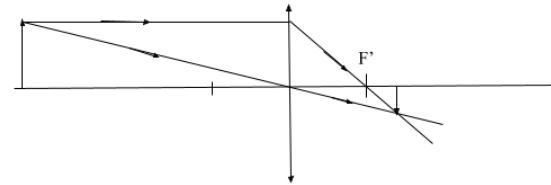
\includegraphics[scale=0.9]{../figs//VN11-2021-PH-TP028-22.JPG}
		\end{center}
				

	}
	\item \mkstar{2} [9]
	
	\cauhoi{
		Một vật sáng AB đặt thẳng góc với trục chính của một thấu kính phân kì có tiêu cự $f$, cách thấu kính một khoảng $\SI{60}{cm}$ cho ảnh A’B’ nhỏ hơn vật 4 lần. Xác định tiêu cự của thấu kính trên. Vẽ hình.
		
	}
	\loigiai{
		
		Đây là thấu kính phân kì nên ảnh là ảnh ảo.
		
		$$k > 0 \Rightarrow k = \dfrac{1}{4} = - \dfrac{d'}{d} \Rightarrow d' = - \SI{15}{cm}.$$
		
		Tiêu cự của thấu kính
		
		$$\dfrac{1}{f} =\dfrac{1}{d} + \dfrac{1}{d'} \Rightarrow f = -\SI{20}{cm}.$$
		
		\begin{center}
			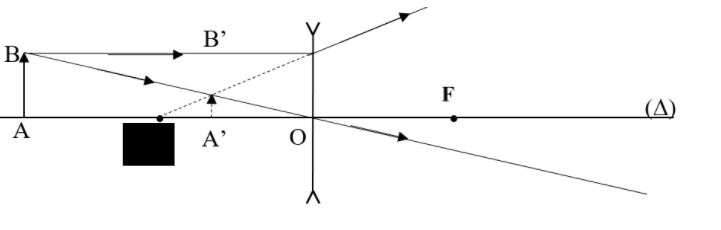
\includegraphics[scale=0.9]{../figs//VN11-2021-PH-TP028-23.JPG}
		\end{center}
	}
		\item \mkstar{2} [13]
	
	\cauhoi{
		
		Cho xy là trục chính của thấu kính phân kỳ, AB là vật sáng, F và F' là các tiêu điểm chính. Hãy vẽ ảnh A'B' của vật AB cho bởi thấu kính. Ảnh A'B' là ảnh thật hay ảnh ảo và có độ lớn như thế nào so với vật AB?
		
		\begin{center}
			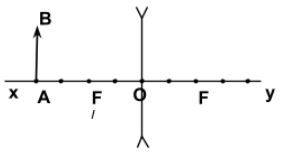
\includegraphics[scale=0.9]{../figs//VN11-2021-PH-TP032-03.JPG}
		\end{center}
	}
	\loigiai{
		
		Thấu kính phân kỳ cho ảnh ảo, cùng chiều và bé hơn vật.
		
		
		\begin{center}
			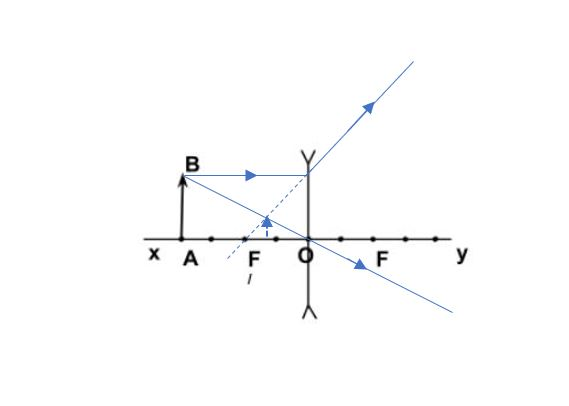
\includegraphics[scale=0.9]{../figs//VN11-2021-PH-TP032-13.JPG}
		\end{center}
	}
	\item \mkstar{2} [24]
	
	\cauhoi{
		Vật sáng AB  được đặt vuông góc với trục chính của một thấu kính hội tụ có tiêu cự $\SI{20}{cm}$ và cách thấu kính $\SI{60}{cm}$. Xác định vị trí, tính chất, chiều và độ lớn của ảnh A$_1$B$_1$ qua thấu kính. Vẽ hình.
		
	}
	\loigiai{
		
		Vị trí của ảnh
		
		$$d'= \dfrac{df}{d-f}=\SI{30}{cm} >0.$$
		
		Suy ra ảnh là ảnh thật, ngược chiều.
		
		Độ phóng đại
		
		$$ k =-\dfrac{d'}{d} = - \dfrac{1}{2}.$$
		
		Ảnh có độ lớn bằng một nửa vật.
		
		\begin{center}
			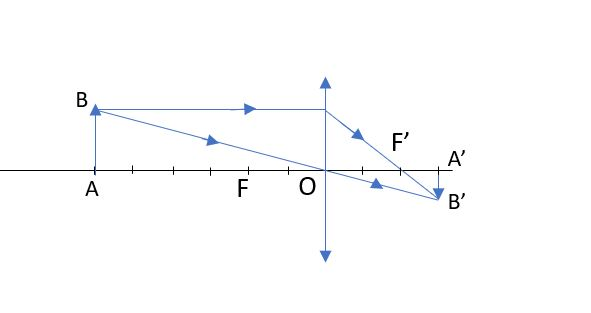
\includegraphics[scale=0.9]{../figs//VN11-2021-PH-TP032-14.JPG}
		\end{center}
	}
	\item \mkstar{2} [25]
	
	\cauhoi{
		
		Vật sáng AB bằng $\SI{2}{cm}$ đặt vuông góc với trục chính của thấu kính hội tụ có tiêu cự $f = \SI{40}{cm}$, cách thấu kính một khoảng $\SI{50}{cm}$. Xác định vị trí, tính chất và độ lớn ảnh A’B’ của AB qua thấu kính. Vẽ hình.
		
		
	}
	\loigiai{
		
		Ta có: 
		
		$$d' = \dfrac{df}{d-f} = \SI{200}{cm.}$$
		
		Độ phóng đại 
		
		$$k = - \dfrac{d'}{d} =-4.$$
		
		Ảnh là ảnh thật, ngược chiều vật, cao gấp 4 lần vật.
		
		\begin{center}
			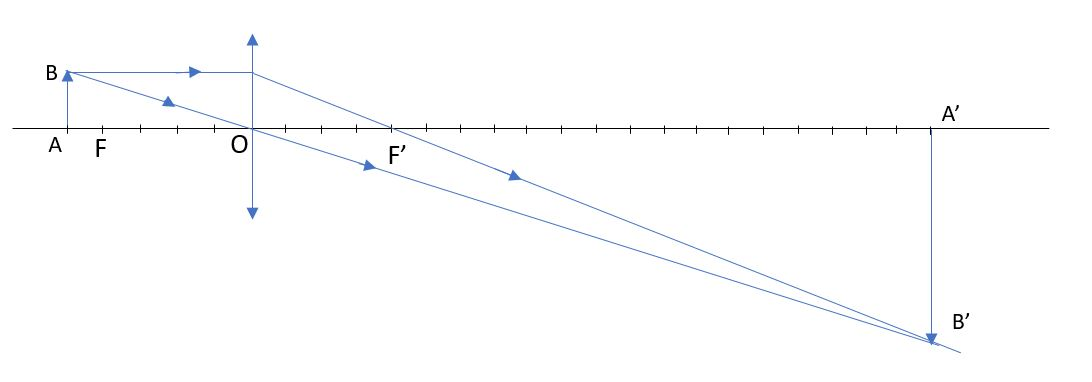
\includegraphics[scale=0.6]{../figs//VN11-2021-PH-TP032-15.JPG}
		\end{center}
	}
	
	
	
	
	\item \mkstar{2} [26]
	
	\cauhoi{
		Vật sáng AB đặt vuông góc với trục chính của một thấu kính hội tụ, cách thấu kính $\SI{12}{cm}$, cho ảnh ảo A$_1$B$_1$. Ảnh này cao gấp 2 lần vật. Xác định tiêu cự của thấu kính.
		
		
	}
	\loigiai{
		
		Ta có:
		
		$$ |k| = \left| - \dfrac{d'}{d}\right| = \dfrac{A_1B_1}{AB} =2.$$
		
		Mà vật thật, ảnh ảo
		
		$$ k = - \dfrac{d'}{d} = 2 \Rightarrow d' =-2d = -\SI{24}{cm}.$$
		
		Tiêu cự của thấu kính
		
		$$\dfrac{1}{f} = \dfrac{1}{d} + \dfrac{1}{d'} \Rightarrow f =\SI{24}{cm}.$$
	}
	\item \mkstar{3} [37]
	
	\cauhoi{
		
		Cho thấu kính hội tụ có tiêu cự $\SI{20}{cm}$. Vật sáng AB là một đoạn thẳng cao $\SI{2}{cm}$ đặt vuông góc trục chính của thấu kính, cách thấu kính $\SI{30}{cm}$. 
		
		\begin{enumerate}[label=\alph*)]
			\item Hãy tính độ tụ của thấu kính trên.
			\item Hãy xác định vị trí ảnh, tính chất ảnh, số phóng đại ảnh và độ cao ảnh. Vẽ hình đúng tỷ lệ.  
			\item Thay thấu kính trên bằng một thấu kính khác sao cho khi  AB cách thấu kính một đoạn $\SI{10}{cm}$ ta thu được ảnh ảo cao $\SI{6}{cm}$. Đây là thấu kính loại gì? Tại sao? Có tiêu cự bằng bao nhiêu?   
		\end{enumerate}
	}
	\loigiai{
		
		\begin{enumerate}[label=\alph*)]
			\item Độ tụ của thấu kính
			
			$$D = \dfrac{1}{f} = \SI{5}{dp}.$$
			
			\item Ta có:
			
			$$\dfrac{1}{f}=\dfrac{1}{d} + \dfrac{1}{d'} \Rightarrow d' = \SI{60}{cm} > 0.$$
			
			Suy ra ảnh là ảnh thật.
			
			Lại có:
			
			$$k = - \dfrac{d'}{d} = -2.$$
			
			Suy ra: 
			
			$$\text{A'B'} = |k| \text{AB} = \SI{4}{cm}.$$
			
			\begin{center}
				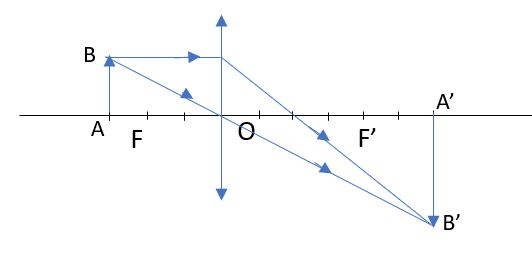
\includegraphics[scale=0.8]{../figs//VN11-2021-PH-TP032-16.JPG}
			\end{center}
			
			\item Vì ảnh ảo cao hơn vật nên đây là thấu kính hội tụ $\text{AB} = \SI{2}{cm}$ và $\text{A'B'} = \SI{6}{cm}.$
			
			Suy ra:
			
			$$ k = 3 = - \dfrac{d'}{d} = \dfrac{f}{d-f}.$$
			
			Giải phương trên ta có $$f= \SI{15}{cm}.$$
			
		\end{enumerate}      
	}
	\item \mkstar{3} [36]
	
	\cauhoi{
		
		Một thấu kính hội tụ có tiêu cự $\SI{6}{cm}$. Vật sáng AB cao $\SI{2}{cm}$ đặt vuông góc với trục chính của thấu kính và cách thấu kính $\SI{8}{cm}$.
		
		\begin{enumerate}[label=\alph*)]
			\item Hãy xác định vị trí, tính chất và độ cao ảnh A’B’ của AB qua thấu kính?
			\item Giữ nguyên vật AB, vị trí của vật và thấu kính. Để thu được ảnh ảo cao gấp 3 lần vật thì ta phải thay thấu kính trên bằng một thấu kính có tiêu cự bằng bao nhiêu ?
		\end{enumerate} 

	}
	\loigiai{
		
	\begin{enumerate}[label=\alph*)]
		\item Ta có: 
		
		$$\dfrac{1}{f} = \dfrac{1}{d} + \dfrac{1}{d'} \Rightarrow d' = \SI{24}{cm} >0 \Rightarrow \text{ảnh thật}.$$
		
		Độ phóng đại
		
		$$ k = - \dfrac{d'}{d} = -3.$$
		
		Mà 
		
		$$|k| = \dfrac{\text{A'B'}}{\text{AB}} \Rightarrow \text{A'B'} = \SI{6}{cm}.$$
		
		Vậy ảnh thu được là ảnh thật, cao $\SI{6}{cm}$ và cách thấu kính $\SI{24}{cm}.$
	
		\item Ta có: 
		
		$$|k_1| = \dfrac{\text{A'B'}}{\text{AB}} =3.$$
		
		Vậy $k_1 =3 \Rightarrow 3 = - \dfrac{d'}{d} \Rightarrow d' = -\SI{24}{cm}.$
		
		Mà
		
		$$\dfrac{1}{f_1} = \dfrac{1}{d} + \dfrac{1}{d'} \Rightarrow f_1 =\SI{12}{cm}.$$ 
	
	\end{enumerate}
	}
	\item \mkstar{3} [35]
	
	\cauhoi{
		 Một vật sáng AB hình mũi tên cao $\SI{2}{cm}$ đặt vuông góc với trục chính của thấu kính (A trên trục chính) cách thấu kính một đoạn $d$.
		 \begin{enumerate}[label=\alph*)]
		 	\item Khi vật AB cách thấu kính một đoạn $d = \SI{15}{cm}$, qua thấu kính cho 1 ảnh thật cao $\SI{4}{cm}$. Xác định loại thấu kính. Tính tiêu cự và độ tụ của thấu kính. Vẽ hình minh họa. 
		 	\item Từ vị trí vật ở câu a, dịch chuyển vật dọc theo trục chính của thấu kính một đoạn thì thu được một ảnh ảo, cao gấp 2 lần vật. Hãy xác định vị trí mới của vật và ảnh. 
		 \end{enumerate}
		
		
	}
	\loigiai{
		\begin{enumerate}[label=\alph*)]
			\item Thấu kính hội tụ: Vì vật thật cho ảnh thật, ảnh lớn hơn vật nên ảnh sẽ ngược chiều vật.
			
			$$k = \dfrac{\text{A'B'}}{\text{AB}} = - 2 = -\dfrac{d'}{d} \Rightarrow   d' =2d =\SI{30}{cm}.$$
			
			Tiêu cự của thấu kính
			
			$$f = \dfrac{d'd}{d+d'} = \SI{10}{cm}.$$
			
			Độ tụ của thấu kính
			
			$$D = \dfrac{1}{f} = \SI{10}{dp}.$$
			
			\begin{center}
				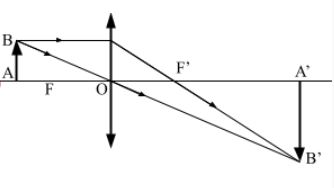
\includegraphics[scale=0.9]{../figs//VN11-2021-PH-TP032-01.JPG}
			\end{center}
			\item Ảnh cùng chiều với vật thật là ảnh ảo: $k = 2$.
			
			Ta có:
			
			$$k = 2 = - \dfrac{d'}{d}\ (1).$$
			
			Và:
			
			$$\dfrac{1}{f} = \dfrac{1}{d} + \dfrac{1}{d'}\ (2).$$
			
			Vị trí vật:
			
			$$\dfrac{1}{f} = \dfrac{1}{d} - \dfrac{1}{2d} = \dfrac{1}{2d} \Rightarrow d = \SI{5}{cm}.$$
			
			Vị trí ảnh: 
			
			$$d' = -2d = -\SI{10}{cm}.$$
			
		\end{enumerate}
		 
	}
	\item \mkstar{3} [34]
	
	\cauhoi{
		
		Một thấu kính phân kỳ có tiêu cự $-\SI{40}{cm}$. Vật sáng $\text{AB} = \SI{2,4}{cm}$ đặt vuông góc trục chính và cách thấu kính một đoạn $\SI{20}{cm}$. Xác định vị trí, tính chất, chiều và độ lớn ảnh và vẽ ảnh.
		
		
	}
	\loigiai{
		
		Vị trí ảnh 
		
		$$ \dfrac{1}{d'} = \dfrac{1}{f} - \dfrac{1}{d} \Rightarrow d = -\dfrac{40}{3}.$$.
		
		Độ phóng đại của thấu kính
		
		$$ k  = -\dfrac{d'}{d} = \dfrac{2}{3}.$$
		
		Do thấu kính phân kỳ nên ảnh là ảnh ảo, cùng chiều và bằng  $\dfrac{2}{3}$ vật.
		
		\begin{center}
			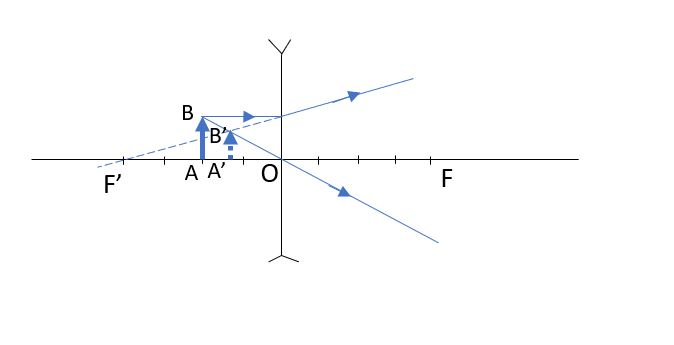
\includegraphics[scale=0.9]{../figs//VN11-2021-PH-TP032-17.JPG}
		\end{center}
	}
	\item \mkstar{3} [11]
	
	\cauhoi{
		
		Một thấu kính hội tụ có độ tụ $\SI{2}{dp}$. 
		\begin{enumerate}[label=\alph*)]
			\item Tính tiêu cự của thấu kính. 
			\item Một vật thật AB cao $\SI{6}{cm}$ đặt vuông góc với trục chính của thấu kính, cách thấu kính $\SI{20}{cm}$. Xác định vị trí, tính chất và chiều cao của ảnh tạo bởi thấu kính.
		\end{enumerate}
		
	}
	\loigiai{
		
			\begin{enumerate}[label=\alph*)]
				
			\item Tiêu cự của thấu kính
			
			$$f=\dfrac{1}{D} = \SI{0,5}{m} = \SI{50}{cm}.$$
			
			\item Khoảng cách từ ảnh đến quang tâm
			
			$$d'=\dfrac{df}{d-f}= -\dfrac{100}{3}\ \text{cm}.$$
			
			A’B’ là ảnh ảo cách thấu kính $\dfrac{100}{3}\ \text{cm}.$
			
			Số phóng đại ảnh: $$k=-\dfrac{d'}{d}=\dfrac{5}{3}.$$
			
			Chiều cao ảnh là $$\text{A’B’} = |k| \text{AB} = \SI{10}{cm}.$$
			
			\end{enumerate}
		
	}
	\item \mkstar{3} [12]
	
	\cauhoi{
		
		Vật sáng AB có điểm A nằm trên trục chính và vuông góc với trục chính của một thấu kính hội tụ. Vật AB cách thấu kính $\SI{40}{cm}$ ta thu được ảnh thật cao bằng nửa vật.
		\begin{enumerate}[label=\alph*)]
			\item Xác định vị trí ảnh và tiêu cự của thấu kính. 
			
			\item Vẽ ảnh A’B’ thu được qua thấu kính.
		\end{enumerate}
		
	}
	\loigiai{
		
		\begin{enumerate}[label=\alph*)]
			\item Vì ảnh thật (ngược chiều) bằng nửa vật nên $k < 0$
			
			$$\Rightarrow   k = - \text{0,5}.$$  
			
			Ta có:
			
			$$k = -\dfrac{d'}{d} \Rightarrow d’= \SI{20}{cm}.$$
			
			Tiêu cực của thấu kính
			
			$$\dfrac{1}{f} = \dfrac{1}{d} + \dfrac{1}{d'} \Rightarrow f =\dfrac{40}{3}\ \text{cm} = \SI{13,33}{cm}.$$
			
			\item Hình vẽ
			
			\begin{center}
				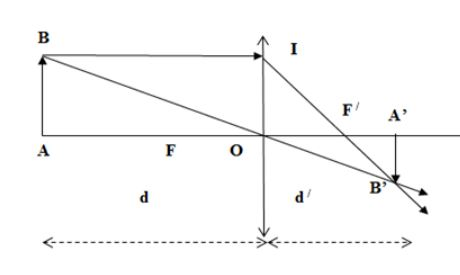
\includegraphics[scale=0.9]{../figs//VN11-2021-PH-TP032-02.JPG}
			\end{center}
		\end{enumerate}
	}

	\item \mkstar{3} [14]
	
	\cauhoi{
		
		Vật sáng AB cao $\SI{4}{cm}$ đặt vuông góc với trục chính của một thấu kính hội tụ có tiêu cự $\SI{20}{cm}$ và cách thấu kính $\SI{10}{cm}$.
		\begin{enumerate}[label=\alph*)]
			\item Tìm khoảng cách từ ảnh tới thấu kính. Tính số phóng đại ảnh và độ cao của ảnh.
			
			\item  Nêu tính chất ảnh. Vẽ hình đúng tỉ lệ.
		\end{enumerate}
		
	}
	\loigiai{
		
		\begin{enumerate}[label=\alph*)]
			\item Vị trí ảnh:
			
			$$d' = \dfrac{df}{d-f} =-\SI{20}{cm}.$$
			
			Hệ số phóng đại:
			
			$$ k = - \dfrac{d'}{d} = 2.$$
			
			Độ cao ảnh
			
			$$\text{A'B'} =|k| \text{AB} = \SI{4}{cm}.$$
			\item 
			Thấu kính hội tụ có $d < f$ nên cho ảnh ảo, cùng chiều và lớn hơn vật.
			\begin{center}
				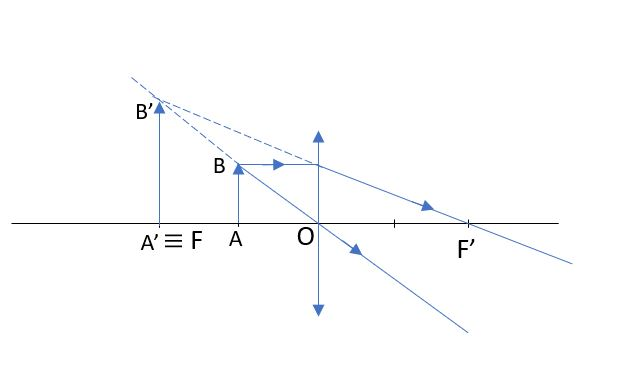
\includegraphics[scale=0.9]{../figs//VN11-2021-PH-TP032-18.JPG}
			\end{center}
		\end{enumerate}
	}

	\item \mkstar{3} [16]
	
	\cauhoi{
		
		 Một thấu kính hội tụ có tiêu cự $\SI{40}{cm}$. Vật sáng AB cao $\SI{10}{cm}$ đặt vuông góc với trục chính của thấu kính và cách thấu kính $\SI{60}{cm}$. Hãy:
	\begin{enumerate}[label=\alph*)]
		\item Xác định vị trí, tính chất, độ cao của ảnh qua thấu kính.
		\item Dựng ảnh của vật sáng AB qua thấu kính.
	\end{enumerate}
		
	}
	\loigiai{
		
		\begin{enumerate}[label=\alph*)]
			\item Xác định vị trí, tính chất, độ cao của ảnh qua thấu kính:
			
			- Vị trí ảnh:
			
			$$\dfrac{1}{f} = \dfrac{1}{d} + \dfrac{1}{d'} \Rightarrow d' = \SI{120}{cm}.$$
			
			- Độ phóng đại:
			
			$$ k =-\dfrac{d'}{d} = -2 <0.$$
			
			Suy ra đây là ảnh thật, ngược chiều.
			
			- Độ cao ảnh
			
			$$\text{A'B'} = |k| \text{AB} = \SI{20}{cm}.$$
			
			
			\item Dựng ảnh của vật sáng qua thấu kính hội tụ:
			
			\begin{center}
				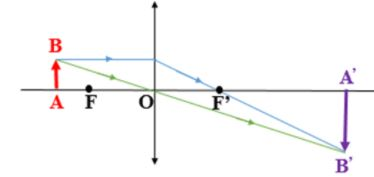
\includegraphics[scale=0.9]{../figs//VN11-2021-PH-TP032-04.JPG}
			\end{center}
		\end{enumerate}
	}
	\item \mkstar{3} [16]
	
	\cauhoi{
		
		 Đặt một vật sáng AB trước một thấu kính có tiêu cự $|f| = \SI{60}{cm}$ và vuông góc với trục chính. Cho biết khoảng cách từ ảnh đến thấu kính là $-\SI{30}{cm}$. Gọi $\overline{A_1B_1}$ là độ cao của ảnh cho bởi thấu kính hội tụ, $\overline{A_2B_2}$ là độ cao của ảnh cho bởi thấu kính phân kỳ. Hãy xác định tỉ số $\dfrac{\overline{A_2B_2}}{\overline{A_1B_1}}$.
		
		
	}
	\loigiai{
		
		* Ảnh tạo bởi thấu kính hội tụ: ($f > 0, f = \SI{60}{cm}$).
		
		Ta có:
		
		$$\dfrac{1}{f} =\dfrac{1}{d} + \dfrac{1}{d'} \Rightarrow d = \SI{20}{cm}.$$
		
		Số phóng đại:
		
		$$k = -\dfrac{d'}{d} = \dfrac{3}{2},$$
		
		Vậy:
		
		$$\overline{A_1B_1} =|k| \overline{AB} = \dfrac{3}{2}\overline{AB}.$$
		
		* Ảnh tạo bởi thấu kính phân kỳ: ($f < 0, f = -\SI{60}{cm}$)
		
		Ta có:
		
		$$\dfrac{1}{f} =\dfrac{1}{d} + \dfrac{1}{d'} \Rightarrow d = \SI{60}{cm}.$$
		
		Số phóng đại:
		
		$$k = -\dfrac{d'}{d} = \dfrac{1}{2},$$
		
		Vậy: $$\overline{A_2B_2} =|k| \overline{AB} = \dfrac{1}{2}\overline{AB}.$$
		
		Tỉ số: $\dfrac{\overline{A_2B_2}}{\overline{A_1B_1}} = \dfrac{1}{3}.$
	}
	\item \mkstar{3} [17]
	
	\cauhoi{
		Một vật sáng AB cao $\SI{3}{cm}$ nằm vuông góc với trục chính của một thấu kính hội tụ và cách thấu kính một khoảng $\SI{60}{cm}$. Tiêu cự của thấu kính là $\SI{20}{cm}$.
		\begin{enumerate}[label=\alph*)]
			\item Tính độ tụ thấu kính.
			\item Tính khoảng cách từ ảnh đến vật. 
			\item Tính độ phóng đại $k$ và cho biết tính chất của ảnh.
			\item Tìm chiều cao của ảnh A’B’.
			\item Vẽ hình đúng tỉ lệ.
		\end{enumerate}
		
	}
	\loigiai{
		
		\begin{enumerate}[label=\alph*)]
			\item Độ tụ của thấu kính
			
			$$D=\dfrac{1}{f}=\SI{5}{dp}.$$
			
			\item Khoảng cách từ ảnh đến vật 
			
			$$d'=\dfrac{df}{d-f} = \SI{30}{cm}.$$
			
			\item Độ phóng đại $k$
			
			$$k=-\dfrac{d'}{d} = - \text{0,5}.$$
			
			Suy ra ảnh thật, ngược chiều.
			\item Chiều cao của ảnh A'B'
			
			$$\text{A'B'}=|k| \text{AB} = \SI{1,5}{cm}.$$
			\item Hình vẽ
			
			\begin{center}
				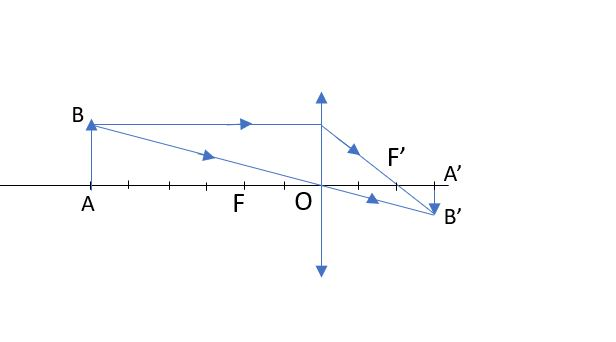
\includegraphics[scale=0.9]{../figs//VN11-2021-PH-TP032-19.JPG}
			\end{center}
		\end{enumerate}
	}
	\item \mkstar{3} [18]
	
	\cauhoi{
		Một vật nhỏ, phẳng AB được đặt trên trục chính và vuông góc với trục chính của một thấu kính hội tụ có tiêu cự $\SI{20}{cm}$. Vật AB đặt cách thấu kính $\SI{30}{cm}$. 
		\begin{enumerate}[label=\alph*)]
			\item Xác định vị trí ảnh, tính chất của ảnh.
			\item Tìm số phóng đại của ảnh. So sánh chiều và độ lớn của ảnh so với vật. Vẽ ảnh.
		\end{enumerate}
		
	}
	\loigiai{
		
		Cho $f = \SI{20}{cm}, d= \SI{30}{cm}.$
		
		\begin{enumerate}[label=\alph*)]
			\item Vị trí ảnh,tính chất của ảnh
			
			$$\dfrac{1}{f} = \dfrac{1}{d} + \dfrac{1}{d'} \Rightarrow d' = \SI{60}{cm} >0.$$
			
			Ảnh A’B’ thật cách thấu kính $\SI{60}{cm}$.
		
			\item Số phóng đại $$k=-\dfrac{d’}{d} = -2. $$
			
			Ảnh A’B’ ngược chiều, lớn gấp 2 lần vật cách thấu kính $\SI{60}{cm}$.
			
			 
			\begin{center}
				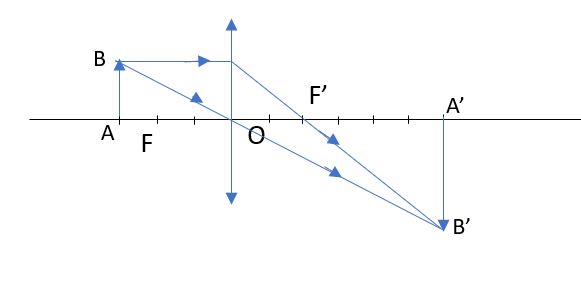
\includegraphics[scale=0.9]{../figs//VN11-2021-PH-TP032-20.JPG}
			\end{center}
			
		\end{enumerate}
	}
	\item \mkstar{3} [19]
	
	\cauhoi{
		Một thấu kính có độ tụ $\SI{2}{dp}$. Vật sáng AB đặt vuông góc với trục chính thấu kính (A nằm trên trục chính) cách thấu kính $\SI{60}{cm}$.
		\begin{enumerate}[label=\alph*)]
			\item Tính tiêu cự của thấu kính.
			\item Tính khoảng cách từ ảnh của AB đến thấu kính. Ảnh là ảnh thật hay ảnh ảo và cao gấp mấy lần vật AB. 
		\end{enumerate}
	}
	\loigiai{
		
		\begin{enumerate}[label=\alph*)]
			\item Tiêu cự của thấu kính
			
			$$f = \dfrac{1}{D} = \SI{0,5}{m}.$$
			
			\item Khoảng cách từ ảnh của AB đến thấu kính
			
			$$d' = \dfrac{df}{d-f} = \SI{3}{m}.$$
			
			$$ k= - \dfrac{d'}{d} = -5< 0.$$ 
			
			Ảnh là ảnh thật và cao gấp 5 lần vật.
		\end{enumerate}
	}
	\item \mkstar{3} [20]
	
	\cauhoi{
		
		Thấu kính hội tụ có độ tụ là $\SI{5}{dp}$.
	\begin{enumerate}[label=\alph*)]
		\item Tìm tiêu cự của thấu kính.
		\item Vật thật đặt trước thấu kính (vuông góc với trục chính của thấu kính) cho ảnh thật bằng 2 lần vật. Hãy xác định vị trí vật và vị trí ảnh. Vẽ hình đúng tỷ lệ. 
	\end{enumerate}
		
	}
	\loigiai{
		
		\begin{enumerate}[label=\alph*)]
			\item Tiêu cự của thấu kính
			
			$$f = \dfrac{1}{D} = \SI{20}{cm}.$$
			
			\item Độ phóng đại
			
			$$ k = - \dfrac{d'}{d} =-2 \Rightarrow d' = -2d.$$
			
			Thế vào công thức 
			
			$$\dfrac{1}{f} = \dfrac{1}{d} +\dfrac{1}{d'} \Rightarrow d = \SI{30}{cm}.$$
			
			$$\Rightarrow d' = \SI{60}{cm}.$$
			
			\begin{center}
				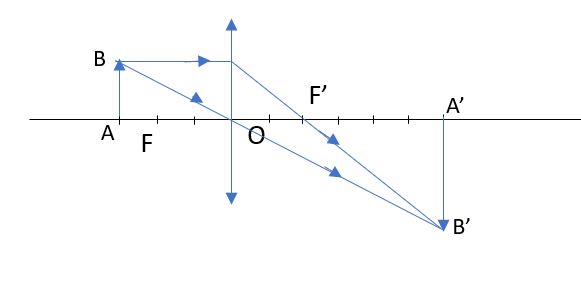
\includegraphics[scale=0.9]{../figs//VN11-2021-PH-TP032-20.JPG}
			\end{center}
		\end{enumerate}
	}

	\item \mkstar{3} [21]
	
	\cauhoi{
		Một vật sáng AB cao $\SI{1}{cm}$ được đặt vuông góc với trục chính của một thấu kính hội tụ cho một ảnh thật A$_1$B$_1$ hiện rõ nét trên màn đặt cách thấu kính $\SI{60}{cm}$ và ảnh này cao $\SI{3}{cm}$. Tìm tiêu cự.
	}
	\loigiai{
		
		Thấu kính hội tụ cho ảnh thật, ngược chiều vật.
		
		Độ phóng đại của thấu kính
		
		$$ k = - \dfrac{d'}{d} = - 3.$$
		
		Vị trí của ảnh
		
		$$ d + d' = \SI{60}{cm}.$$
		
		Suy ra: $d = \SI{15}{cm}$; $d' = \SI{45}{cm}.$
		
		Tiêu cự của thấu kính
		
		$$\dfrac{1}{f} = \dfrac{1}{d} + \dfrac{1}{d'} \Rightarrow f = \SI{11,25}{cm}. $$
		
	}

		\item \mkstar{3} [22]
	
	\cauhoi{
		
		Vật sáng AB cao $\SI{2}{cm}$ đặt vuông góc với trục chính của một thấu kính hội tụ có tiêu cự $\SI{36}{cm}$, vật cách thấu kính $\SI{60}{cm}$. Xác định vị trí, độ phóng đại, chiều cao ảnh A$_1$B$_1$ của vật AB cho bởi thấu kính. 
	}
	\loigiai{
		
		Vị trí ảnh
		
		$$d'  = \dfrac{df}{d-f} = \SI{90}{cm}.$$
		
		Độ phóng đại 
		
		$$ k = - \dfrac{d'}{d} = -\text{1,5}.$$
		
		Chiều cao của ảnh A$_1$B$_1$
		
		$$ A_1B_1 = |k| AB =\SI{3}{cm}.$$
		
		
	}
	\item \mkstar{3} [23]
	
	\cauhoi{
		Một thấu kính hội tụ có độ tụ $D = \SI{5}{dp}$. Đặt một vật sáng AB có chiều cao $\SI{2}{cm}$ trước thấu kính $\SI{40}{cm}$.
		
		\begin{enumerate}[label=\alph*)]
			\item Xác định tiêu cự của thấu kính.
			\item Xác định vị trí, độ phóng đại, độ cao của ảnh.
		\end{enumerate}
	}
	\loigiai{
		
		\begin{enumerate}[label=\alph*)]
			\item Tiêu cự của thấu kính
			
			$$ f=\dfrac{1}{D} = \SI{20}{cm}.$$
			
			\item Vị trí của vật
			
			$$\dfrac{1}{f} = \dfrac{1}{d} + \dfrac{1}{d'} \Rightarrow d' = \SI{40}{cm}.$$
			
			Độ phóng đại 
			
			$$ k  = -\dfrac{d'}{d} =-1.$$
			
			Chiều cao của ảnh
			
			$$\text{A'B'} = |k|\text{AB} =\SI{2}{cm}.$$
			
			
		\end{enumerate}
		
	}
	
	
	\item \mkstar{3} [27]
	
	\cauhoi{
		Cho một vật sáng AB cao $\SI{2}{cm}$ đặt vuông góc với trục chính của một thấu kính hội tụ có tiêu cự $\SI{25}{cm}$. 
		
		\begin{enumerate}[label=\alph*)]
			\item Tính độ tụ của thấu kính.
			\item Biết vật AB đặt cách thấu kính $\SI{15}{cm}$. Xác định vị trí, tính chất và chiều cao ảnh. 
		\end{enumerate}
		
	}
	\loigiai{
		
		\begin{enumerate}[label=\alph*)]
			\item Độ tụ của thấu kính
			
			$$ D = \dfrac{1}{f} = \SI{4}{dp}.$$
			\item Ta có:
			
			$$\dfrac{1}{f} = \dfrac{1}{d} + \dfrac{1}{d'} \Rightarrow d' =-\SI{37,7}{cm}.$$
			
			Độ phóng đại của thấu kính
			
			$$ k = - \dfrac{d'}{d} = -\text{2,5}.$$
			
			Chiều cao của ảnh
			
			$$\text{A'B'} = |k|AB = \SI{5}{cm}.$$
			
			
		\end{enumerate}
	}
\end{enumerate}	
\section{Lý thuyết: Dời vật hoặc thấu kính}
\begin{enumerate}[label=\bfseries Câu \arabic*:]
		\item \mkstar{3} [6]
	
	\cauhoi{
		Vật sáng AB đặt vuông góc với trục chính của một thấu kính có tiêu cự $\SI{30}{cm}$ cho ảnh A’B’ = 3AB rõ nét trên màn. Để thu được ảnh A’B’ = 0,5AB trên  màn  ta phải di chuyển vật sáng  đến gần hay ra xa một đoạn là bao nhiêu?
	}
	\loigiai{
		
		Cho ảnh thật $k= -3$
		
		$$k =-\dfrac{d'}{d}= -3 \Rightarrow d'=3d.$$
		
		Lại có:
		
		$$\dfrac{1}{f} = \dfrac{1}{d}+ \dfrac{1}{d'} \Rightarrow d = \SI{40}{cm}; d' =\SI{120}{cm}.$$
		
		Do ảnh thật nên 
		
		$$ k_1 =-\text{-0,5} = \dfrac{f}{f - d_1} \Rightarrow d_1 = \SI{90}{cm}.$$
		
		Do $d_1 >d$ nên vật di chuyển ra xa một đoạn $\Delta d = 90 -40=\SI{50}{cm}.$
	}
	
		\item \mkstar{3} [21]
	
	\cauhoi{
		Một vật sáng AB cao $\SI{1}{cm}$ được đặt vuông góc với trục chính của một thấu kính hội tụ cho một ảnh thật A$_1$B$_1$ hiện rõ nét trên màn đặt cách thấu kính $\SI{60}{cm}$ và ảnh này cao $\SI{3}{cm}$. Giữ nguyên thấu kính, muốn quan sát được ảnh A$_2$B$_2$ cùng chiều và cách vật AB một đoạn $\SI{20}{cm}$ thì phải dời vật một đoạn bao nhiêu theo chiều nào?   
	}
	\loigiai{
		
		Độ phóng đại của thấu kính
		
		$$ k  =  - \dfrac{d'}{d} = -3.$$
		
		Ta có:
		
		$$d + d' = \SI{60}{cm}.$$
		
		Suy ra $d = \SI{15}{cm}$; $d' = \SI{45}{cm}.$
		
		Tiêu cực của thấu kính
		
		$$f = \dfrac{dd'}{d + d'} = \dfrac{45}{4}\ \text{cm}.$$
		
		Qua thấu kính hội tụ muốn cho ảnh cùng chiều thì là ảnh ảo.
		
		$$ d'_1 - d_1 = \SI{20}{cm}.$$
		
		Lại có:
		
		$$\dfrac{1}{f} = \dfrac{1}{d_1} + \dfrac{1}{d'_1} = \dfrac{4}{45}.$$
		
		Suy ra $d_1=\SI{8}{cm}.$
		
	}
		\item \mkstar{3} [21]
	
	\cauhoi{
		Vật sáng AB  đặt trên trục chính, vuông góc với trục chính của một thấu kính, cho ảnh thật A’B’ rõ nét trên màn.Giữ cố định thấu kính, khi dời vật ra xa thấu kính một đoạn $\SI{2}{cm}$ dọc theo trục chính, và dời màn một đoạn $\SI{30}{cm}$ thì thu được  ảnh rõ  nét trên màn  nhưng ảnh này bằng 0,6  lần ảnh trước. Tìm tiêu cự của thấu kính.
		
		
	}
	\loigiai{
		
		Áp dụng công thức 
		
		$$\dfrac{1}{f}=  \dfrac{1}{d}+\dfrac{1}{d’}$$
		
		$$k=\dfrac{f}{f-d}$$
		
		$$k= \dfrac{f-d’}{f}$$   
		
		Suy ra $f= \SI{15}{cm}.$
	}
		\item \mkstar{3} [22]
	
	\cauhoi{

		Vật sáng AB cao $\SI{2}{cm}$ đặt vuông góc với trục chính của một thấu kính hội tụ có tiêu cự $\SI{36}{cm}$, vật cách thấu kính $\SI{60}{cm}$. Giữ nguyên vị trí thấu kính, dịch  chuyển vật AB sao cho ảnh mới A$_2$B$_2$ cao bằng ảnh A$_1$B$_1$. Hỏi dịch chuyển vật lại gần hay ra xa thấu kính một đoạn bao nhiêu? 
		
	}
	\loigiai{
		
		Vị trí ảnh
		
		$$d'  = \dfrac{df}{d-f} = \SI{90}{cm}.$$
		
		Độ phóng đại 
		
		$$ k = - \dfrac{d'}{d} = -\text{1,5}.$$
		
		Chiều cao của ảnh A$_1$B$_1$
		
		$$ A_1B_1 = |k| AB =\SI{3}{cm}.$$
		
		Ảnh mới A$_2$B$_2$ cao bằng ảnh A$_1$B$_1$. Suy ra ảnh mới A$_2$B$_2$ chỉ là ảnh ảo.
		
		$$k =\text{1,5} = - \dfrac{f}{d_2 - f} \Rightarrow d_2 = \SI{12}{cm}.$$
		
		Dời vật lại gần thấu kính 48 cm.
		
		
	}
		\item \mkstar{3} [24]
	
	\cauhoi{
		Vật sáng AB  được đặt vuông góc với trục chính của một thấu kính hội tụ có tiêu cự $\SI{20}{cm}$ và cách thấu kính $\SI{60}{cm}$. Thay đổi vị trí của vật sáng AB ta có một ảnh khác là A$_2$B$_2$ bằng 0,6 lần vật. Xác định vị trí của vật lúc này.
		
	}
	\loigiai{
		
		Vị trí ảnh
		
		$$\dfrac{1}{d} = \dfrac{1}{f} - \dfrac{1}{d'} \Rightarrow d = \SI{30}{cm}.$$
		
		Độ phóng đại lúc đầu
		
		$$ k = - \dfrac{d'}{d} = - \text{0,5}. \ (1)$$
		
		Độ phóng đại lúc sau
		
		$$k_1 = \dfrac{d'}{d_1} = - \text{0,6}. \ (2)$$
		
		Lấy (1)  chia (2):
		
		$$\dfrac{d_1}{d} = \dfrac{5}{6} \Rightarrow d_1 = \SI{50}{cm}.$$
	}
		\item \mkstar{3} [24]
	
	\cauhoi{
		
	Một vật sáng phẳng AB được đặt trước một thấu kính, vuông góc với trục chính. Ảnh A$_1$B$_1$ của vật tạo bởi thấu kính bằng sáu lần vật. Dời vật lại gần thấu kính một đoạn $\SI{15}{cm}$. Ảnh của vật A$_2$B$_2$ ở vị trí mới vẫn bằng sáu lần vật. Tính tiêu cự của thấu kính.
	
		
	}
	\loigiai{
		
		Từ đề bài suy ra $ k_1 =-6$; $k_2 =6.$
		
		$$k = - \dfrac{f}{d-f} \Rightarrow d =f - \dfrac{f}{k}.$$
		
		$$d_1 =f - \dfrac{f}{k_1}\ (1).$$
		
		$$d_2 = f - \dfrac{f}{k_2}\ (2).$$
		
		$$d_1-d_2 =15\ (3).$$
		
		Kết hợp 1, 2, 3 giải ra $f =\SI{15}{cm}.$
	}
		\item \mkstar{3} [25]
	
	\cauhoi{
		
	Vật sáng AB bằng $\SI{2}{cm}$ đặt vuông góc với trục chính của thấu kính hội tụ có tiêu cự $f = \SI{40}{cm}$, cách thấu kính một khoảng $\SI{50}{cm}$. Để thấu kính cố định, phải tịnh tiến AB dọc theo trục chính như thế nào để ảnh A’B’ của AB qua thấu kính là ảnh thật, nhỏ hơn AB và cách AB một khoảng $\SI{250}{cm}$. 

	}
	\loigiai{
		
		Ta có:
		
		$$d +d' = \SI{250}{cm}.$$
		
		Lại có:
		
		$$ f = \dfrac{dd'}{d + d'}.$$
		
		Suy ra phương trình
		
		$$d^2 - Ld +Lf =0.$$
		
		Có 2 nghiệm 
		
		$$d =\SI{200}{cm} \Rightarrow d' = \SI{50}{cm}\ \text{nhận}.$$
		
		$$d =\SI{50}{cm} \Rightarrow d' = \SI{200}{cm}\ \text{loại}.$$
		
		Vậy dịch chuyển vật ra xa thấu kính một đoạn: 150 cm.
	}
		\item \mkstar{3} [26]
	
	\cauhoi{
		Cho vật thật AB đặt vuông góc với trục chính của một thấu kính hội tụ có tiêu cự $\SI{20}{cm}$. Vật đặt cách thấu kính một khoảng $\SI{30}{cm}$. Sau đó vật di chuyển từ vị trí ban đầu đến vị trí cách thấu kính $\SI{40}{cm}$ với tốc độ trung bình là $\SI{5}{cm/s}$. Xác định tốc độ chuyển dời trung bình của ảnh trong trường hợp trên.
			}
	\loigiai{
		
		+ Vị trí ảnh ban đầu: 
		
		$$\dfrac{1}{f} = \dfrac{1}{d_1} + \dfrac{1}{d'_1} \Rightarrow d'_1 =\SI{60}{cm}.$$
		
		+  Vị trí ảnh lúc sau:
		
		$$\dfrac{1}{f} = \dfrac{1}{d_2} + \dfrac{1}{d'_2} \Rightarrow d'_2 =\SI{40}{cm}.$$
		
		+ Thời gian dịch chuyển của ảnh: 
		
		$$ t = \dfrac{|d_2 - d_1|}{v} = \SI{2}{s}.$$
		
		+ Tốc độ dịch chuyển trung bình của ảnh là:
		
		$$v_\text a = \dfrac{|d'_2 -d'_1|}{t} = \SI{10}{cm/s}.$$
	}
		\item \mkstar{3} [26]
	
	\cauhoi{
		Vật sáng AB đặt vuông góc với trục chính của một thấu kính hội tụ, cách thấu kính $\SI{12}{cm}$, cho ảnh ảo A$_1$B$_1$. Ảnh này cao gấp 2 lần vật. Muốn ảnh A$_2$B$_2$ là ảnh thật, cao bằng ảnh A$_1$B$_1$ thì phải dời vật AB một khoảng bao nhiêu?
	}
	\loigiai{
		
		Ta có:
		
		$$|k'| = \left|-\dfrac{d'_2}{d_2}\right| = \dfrac{A_2B_2}{AB}=2.$$
		
		Mà vật thật, ảnh thật:
		
		$$ k' = - \dfrac{d'_2}{d_2} =-2 \Rightarrow d'_2 =2d_2.$$
		
		Ta có:
		
		$$\dfrac{1}{f} = \dfrac{1}{d_2} + \dfrac{1}{d'_2} \Rightarrow d_2 =\SI{36}{cm}.$$
		
		Độ dịch chuyển của vật
		
		$$\Delta d = |d_2 -d_1| =\SI{24}{cm}.$$
	}

	\item \mkstar{3} [27]
	\cauhoi{
		
		Đặt vật AB vuông góc với trục chính của một thấu kính hội tụ có tiêu cự $\SI{20}{cm}$, đặt vật AB cách thấu kính một khoảng $d$ ta thu được ảnh ngược chiều với vật. Di chuyển vật dọc theo trục chính đến một vị trí khác cho tới khi thu được ảnh hiện ra trước thấu kính, và cách thấu kính $\SI{20}{cm}$. Biết rằng hai ảnh có cùng chiều cao. Hỏi ban đầu, vật cách thấu kính một đoạn bao nhiêu?
		
	}
	\loigiai{
		
		Ta có: $d’_2= -\SI{20}{cm}$ và $d_2 = \SI{10}{cm}$.
		
		Tính được 
		
		$$k_2= \dfrac{d'_2}{d_2}= 2.$$
		
		Suy ra được công thức  
		
		$$k_1= - k_2 = -2.$$
		
		Giải phương trình tính được $d=\SI{30}{cm}.$
		
		
	}

		\item \mkstar{4} [19]
	
	\cauhoi{
		Một thấu kính có độ tụ $\SI{2}{dp}$. Vật sáng AB đặt vuông góc với trục chính thấu kính (A nằm trên trục chính) cách thấu kính $\SI{60}{cm}$. Thay vật AB bằng điểm sáng S đặt trên trục chính, trước thấu kính và cách thấu kính $\SI{75}{cm}$. Phía sau thấu kính, đặt một màn quan sát E vuông góc với trục chính của thấu kính. Tịnh tiến màn ra xa thấu kính thì thấy khi màn cách thấu kính một đoạn $L_1$ và $L_2$ thì vết sáng (xem như tròn) trên màn có đường kính gấp 3 lần nhau. Biết $L_2 - L_1 = \SI{20}{cm}$ và $L_1$, $L_2$ đều có giá trị nhỏ hơn $\SI{150}{cm}$. Tính giá trị của $L_1$ và $L_2$. 
		
	}
	\loigiai{
		\begin{center}
			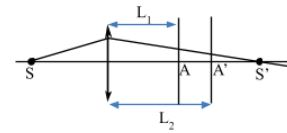
\includegraphics[scale=1]{../figs//VN11-2021-PH-TP032-05.JPG}
		\end{center}
		Ta có:
		
		$$\dfrac{1}{f} = \dfrac{1}{d}+ \dfrac{1}{d'} \Rightarrow d' = \SI{150}{cm}.$$
		
		Lại có:
		
		$$150 - L_1 = 3(150-L_2).$$
		
		Mà $L_2 - L_1 = \SI{20}{cm}.$
		
		Suy ra $L_1 = \SI{120}{cm}; L_2 = \SI{140}{cm}.$
		
		
	}
\end{enumerate}	
\whiteBGstarEnd